\documentclass[final,inline,narroweqnarray,a4paper]{ieee}
% In order to use the figure-defining commands in ieeefig.sty...
\usepackage{ieeefig}
\usepackage[utf8]{inputenc}
\usepackage[spanish]{babel}
\usepackage[T1]{fontenc}
\usepackage{graphicx}
\usepackage{textcomp}
\usepackage{float}
%\usepackage{hyperref}

\begin{document}

%----------------------------------------------------------------------
% Title Information, Abstract and Keywords
%----------------------------------------------------------------------
\title[TP1: Wiretapping]{%
Trabajo Práctico \textnumero 1: Wiretapping}

% format author this way for journal articles.
\author[Alvaro, Barbeito, Brum, Nievas]{%
	Alvaro Jose Fernando, 
    \authorinfo{%
    Alvaro Jose Fernando, LU: \mbox{89/10}, email: \mbox{fer1578@gmail.com}}
	\and
	Barbeito Nicolás,
    \authorinfo{%
    Barbeito Nicolás, LU: \mbox{147/10}, email: \mbox{nicolasbarbeiton@gmail.com}}
	\and
	Brum Raúl,
    \authorinfo{%
    Brum Raúl, LU: \mbox{199/98}, email: \mbox{brumraul@gmail.com}}
	\and
	Nievas Yésica
    \authorinfo{%
    Nievas Yésica, LU: \mbox{340/05}, email: \mbox{yesica.nievas@gmail.com}}
}

% make the title
\maketitle

% do the abstract
\begin{abstract}
Our premise is ...
\end{abstract}

\section{Introducción}\label{sec:intro}

\subsection{Paquetes ARP}
El protocolo ARP (Address Resolution Protocol) permite mapear direcciones de nivel de red a direcciones físicas. La idea de este protocolo se basa en el envío de paquetes que pueden ser de preguntas o respuestas. El emisor del paquete que pregunta por una dirección, envía un mensaje broadcast sobre la red local, siendo respondido por un mensaje unicast por aquel al que pertenece la dirección consultada. Mediante el envío de estos paquetes ARP se construyen las tablas que mapean direcciones de red con direcciones físicas.

\subsection{Entropía de una fuente}
Para poder definir la entropía de una fuente, necesitamos la definición de información que aportan los símbolos emitidos por dicha fuente. Se define información de un símbolo \textit{s} como 
\begin{center}
	I (\textit{s}) = log(1/P(\textit{s})) 
\end{center}
siendo P(\textit{s}) la probabilidad de ocurrencia de dicho símbolo.
De esta manera, puede calcularse la información media suministrada por una fuente de información de memoria nula (los símbolos emitidos son estadísticamente independientes) como 

\begin{center}
$\sum_{S} P(s_{i})I(s_{i}) \forall{s_{i}} \in{S}$
\end{center}

\begin{flushleft}
	Esta cantidad media de información por símbolo de la fuente, recibe el nombre de \textit{entropía} H(S) de la fuente de memoria nula.
\end{flushleft}

\begin{center}
	$H(S) =\sum_{S} P(s_{i})log(1/P(s_{i}))$ 

\end{center}
	
Debido a que la entropía de una fuente depende de la probabilidad de los diferentes símbolos que la componen, se puede demostrar que para una fuente de información de memoria nula con un alfabeto de q símbolos, el valor máximo de la entropía es precisamente log q, alcanzándose solamente si todos los símbolos son equiprobables.


\subsection{Fuente S} \label{ssec:fuenteS}

Sea P la fuente de información generada a partir de todos los paquetes Ethernet que se transmiten en una determinada red entre los instantes de tiempo $[t_{i}, t_{f}]$:

	$P_{ti,tf} = \{p_{1}...p_{n}\}$ 

\begin{flushleft}
	siendo p{\scriptsize \textit{i}} el i-ésimo paquete transmitido en la red entre los instantes de tiempo $[t_{i},t_{f}]$.
\end{flushleft}

Los paquetes $p{\scriptsize \textit{i}}$ pertenecientes a P encapsulan diferentes protocolos, que se pueden identificar a través del campo type del frame de capa 2 (p.type en Scapy). Por lo tanto, con el objetivo de distinguir los protocolos utilizados en una red, se define otra fuente de información S de la siguiente manera:

$S_{ti,tf} = \{s_{1}...s_{n}\}$ 

\begin{flushleft}
	siendo s{\scriptsize \textit{i}} = p{\scriptsize \textit{i}}.type /p{\scriptsize \textit{i}} perteneciente a P entre los instantes de tiempo $[t_{i},t_{f}]$.
\end{flushleft}


\subsection{Propuesta de una nueva fuente S{\scriptsize 1}} \label{ssec:fuenteS1}
Para analizar la entropía de la red en base a los paquetes ARP observados realizamos una nueva tool en base a la anterior que nos permitiera obtener datos de los campos de dichos paquetes. 
	Se propone como nueva fuente S1 el conjunto de símbolos conformado por las distintas direcciones IP destino:\\
	
	
		S{\scriptsize 1} = \{s{\scriptsize 1}{\tiny 1}...s{\scriptsize 1}{\tiny n}\} siendo s{\scriptsize 1}{\tiny i} el valor del campo \textit{pdst} correspondiente a la ip destino del paquete\\
		
	
	Al igual que para la fuente S, realizamos el cálculo de la entropía como fue requerido, como la probabilidad e información de sus símbolos.  

\section{Métodos y condiciones de cada experimento}

En esta sección describiremos brevemente las redes elegidas para realizar las escuchas mediante las herramientas indicadas en el enunciado del trabajo practico.

\subsection{Home Lan}

Esta medición fue realizada en la Lan de una casa por un intervalo de 2 horas. La misma cuenta con una computadora corriendo un sistema operativo Linux la cual es el router de la Lan y provee a las demás computadoras de acceso a internet ademas de otros servicios de red (proxy, dns, dhcpcd, etc). A la misma se encuentran conectadas mediante un switch 4 computadoras cableadas y 2 access point inalambricos. A estos últimos se encontraban conectados al momento de la medición una notebook y varios celulares. Ademas una de las computadoras cableadas corre una maquina virtual con ip propia independiente y otra de las computadoras cableadas posee otro isp para conectarse a internet por lo que no utiliza a la primera computadora como gateway.

\subsection{Labos Dc}

Esta medición fue realizada en los laboratorios del departamento de computación por un intervalo de 30 minutos. Se desconoce la cantidad de computadoras y celulares conectados al momento de realizar la captura.

\subsection{Zona pública (parque)}
Se realizó una medición en un parque con wifi abierto durante 15 minutos. Debido a que la medición fue realizada en un espacio público se espera que varios dispositivos móbiles como celulares y notebooks se conecten a la misma, sin poder precisar cuántos a priori.

\subsection{Universidad (Universidad de la Matanza)}
Esta medición se realizó por aproximadamente 10 minutos en la red wifi de la Universidad de La Matanza. Es una red abierta y desconocemos la estructura de ella.

\section{Resultados y Análisis}
En esta sección mostraremos y analizaremos los resultados obtenidos en las mediciones realizadas en las distintas redes tanto para la fuente $S$ y $S_1$ descriptas en la sección ~\ref{sec:intro} ~\ref{ssec:fuenteS} y ~\ref{ssec:fuenteS1}. Para cada una de las redes veremos sus protocolos distinguidos, la proporción de paquetes ARP en el trafico de la red y los nodos (representados por ip) distinguidos. Cabe aclarar que para la fuente $S_1$ podemos ver todos los pedidos ``who has'' de ARP ya que todas las maquinas están en el mismo dominio de broadcast pero solo podremos ver las respuestas ``is at'' de aquellas maquinas que se encuentren en igual dominio de colisión (generalmente las conectadas por wireless ya que las cableadas al estar conectadas por switches no tienen colisión y solo el destinatario recibirá la respuesta). 


\subsection{Home Lan}
\subsubsection{Fuente S}

Los resultados obtenidos para la fuente $S$ fueron:

\begin{table}[H]
    \begin{center}
        \begin{tabular}{|c|c|c|}
            \hline
            \textbf{Protocolo} & \textbf{Información} & \textbf{Probabilidad} \\ \hline
            \texttt{EAPOL     }& 12.31       & 0.01\%     \\ \hline
            \texttt{ARP       }& 5.11        & 2.88\%     \\ \hline
            \texttt{IPv6      }& 4.22        & 5.33\%     \\ \hline
            \texttt{IPv4      }& 0.12        & 91.76\%    \\ \hline
        \end{tabular}
        \caption{Home Lan - Protocolos}
        \label{table:homelanS}
    \end{center}
\end{table}

Como puede observarse en la figura~\ref{torta:homelanS} el protocolo mas utilizado es IPv4 en un 91.76\% mientras que IPv6 y ARP solo son utilizados en un 5.33\% y 2.88\% respectivamente. EAPOL (autenticación wireless) no tiene prácticamente incidencia.
Observamos ademas que el protocolo ARP tiene solo una incidencia del 2.88\% en el trafico total de la fuente lo que hace que el overhead aportado por el mismo no sea significativo. 

\begin{figure}[H]
    \begin{center}
        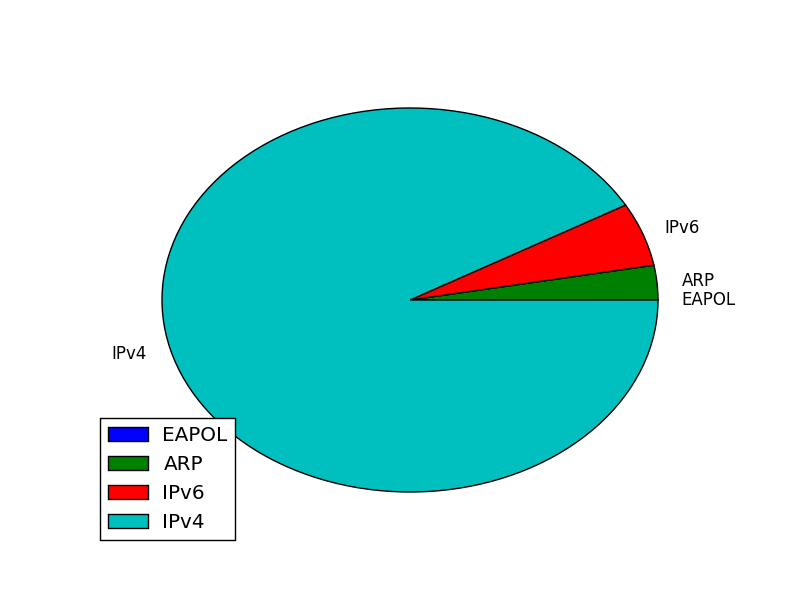
\includegraphics[width=0.5\textwidth]{plot/homelanS-pie.png}
        \caption{Home Lan - Probabilidades}
        \label{torta:homelanS}
    \end{center}
\end{figure}

Por otro lado la entropía de la fuente $S$ fue de 0.4892 lo que hace que los símbolos emitidos por la fuente $S$ sean muy previsibles. Esto podemos notarlo en la figura~\ref{histo:homelanS} donde observamos que el protocolo con mayor porcentaje de aparición, IPv4,  sea el que menos información aporta a la fuente. La información aportada por este se encuentra por debajo de la entropía de $S$. Como contraste observamos en la figura~\ref{histo:homelanS} que el protocolo EAPOL es el que mas información aporta pero según lo observado en la figura~\ref{torta:homelanS} tiene una probabilidad muy baja lo que hace que no incida en la entropía.

\begin{figure}[H]
    \begin{center}
        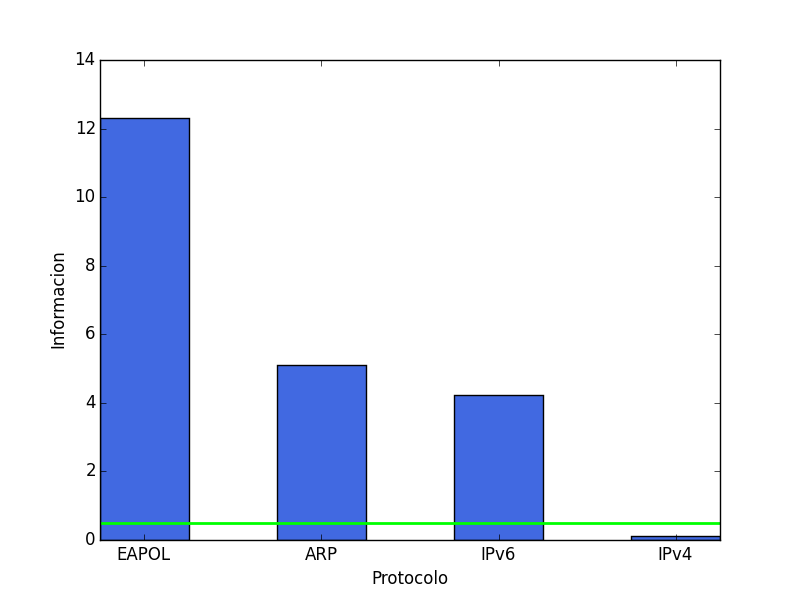
\includegraphics[width=0.5\textwidth]{plot/homelanS-bar.png}
        \caption{Home Lan - Información}
        \label{histo:homelanS}
    \end{center}
\end{figure}

\subsubsection{Fuente $S_1$}
Para la fuente $S_1$ expondremos las ip de destino, los resultados fueron :

\begin{table}[H]
    \begin{center}
        \begin{tabular}{|c|c|c|}
            \hline
            \textbf{Protocolo} & \textbf{Información} & \textbf{Probabilidad} \\ \hline
            \texttt{192.168.10.10}&7.68        & 0.48\%     \\ \hline
            \texttt{192.168.10.27}&6.41        & 1.16\%     \\ \hline
            \texttt{192.168.10.11}&6.30        & 1.26\%     \\ \hline
            \texttt{192.168.10.13}&5.09        & 2.92\%     \\ \hline
            \texttt{192.168.10.7}&4.33         & 4.97\%     \\ \hline
            \texttt{192.168.10.1}&4.00         & 6.23\%     \\ \hline
            \texttt{192.168.10.4}&2.54         & 17.15\%    \\ \hline
            \texttt{192.168.10.6}&2.11         & 23.09\%    \\ \hline
            \texttt{192.168.10.9}&1.22         & 42.69\%    \\ \hline
        \end{tabular}
        \caption{Home Lan - Nodos}
        \label{table:homelanS1}
    \end{center}
\end{table}

Como puede observarse en la figura~\ref{torta:homelanS1} las ip que aparecen con mayor frecuencia como destino en los paquetes ARP son la ``192.168.10.9'' en un 42.69\%, la ``192.168.10.6'' en un 23.09\% y la ``192.168.10.4'' en un 17.15\% por lo que estas serán los nodos distinguidos de la fuente y las que menos información aporten.

\begin{figure}[H]
    \begin{center}
        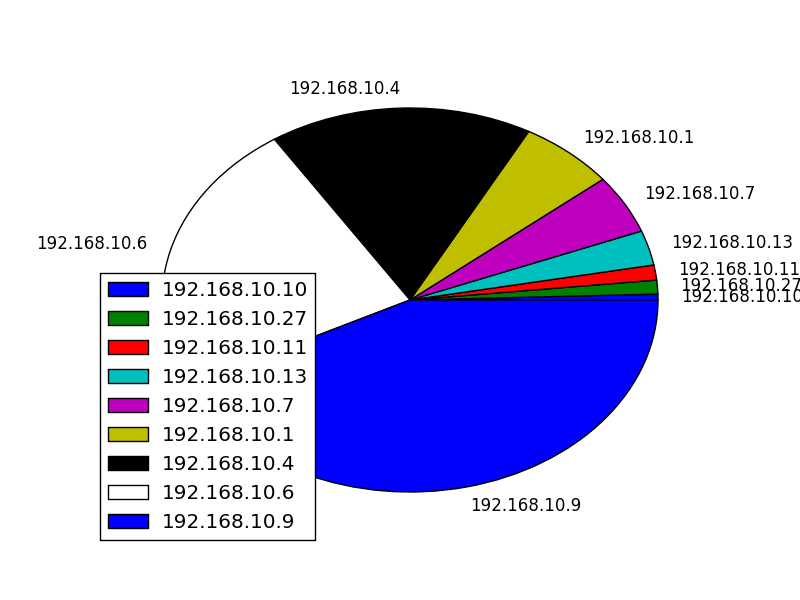
\includegraphics[width=0.5\textwidth]{plot/homelanS1-pie.png}
        \caption{Home Lan - Probabilidades}
        \label{torta:homelanS1}
    \end{center}
\end{figure} 

La entropía de la fuente $S_1$ fue de 2.25. En la figura~\ref{histo:homelanS1} se observa la información aportada por los distintos nodos y como 2 de los nodos distinguidos quedan por debajo de la entropía de la fuente y el otro apenas por arriba. 

\begin{figure}[H]
    \begin{center}
        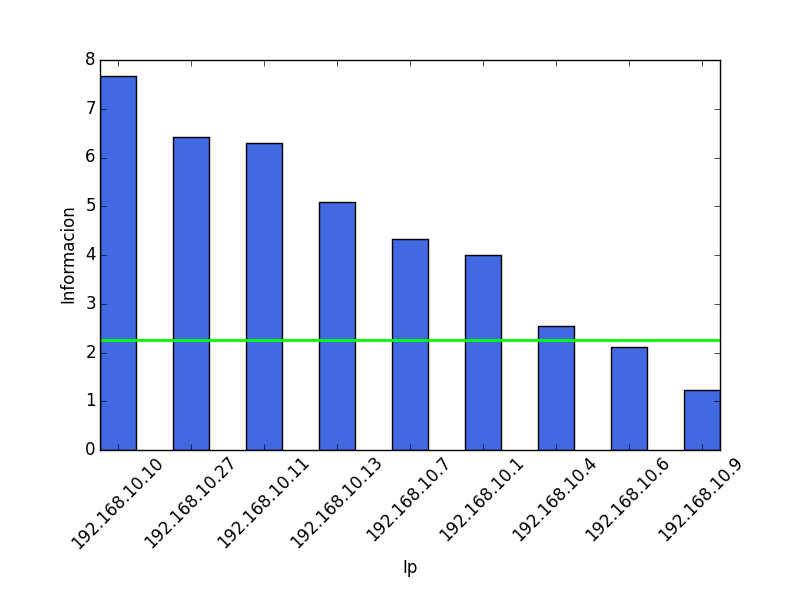
\includegraphics[width=0.5\textwidth]{plot/homelanS1-bar.png}
        \caption{Home Lan - Información}
        \label{histo:homelanS1}
    \end{center}
\end{figure}

En el análisis de la fuente $S_1$ vemos que ninguno de los 3 nodos distinguidos pertenecen al router de la red, la ip ``192.168.10.1''. De los nodos distinguidos las ip ``192.168.10.6'' y ``192.168.10.4'' se explican ya que la primera es la notebook que realizo la captura en la red y la segunda es la computadora que la controlaba remotamente mediante SSH. La ip ``192.168.10.9'' corresponde a la ip de una consola de video juegos la cual se encontraba apagada al momento de realizar la captura, en la ip ``192.168.10.4'' hay un daemon ejecutándose que se comunica con la consola de video juegos. Al estar esta apagada hay muchos pedidos ``who has 192.168.10.9'' y ninguna respuesta por lo que los pedidos son reiterados varias veces incrementado su incidencia.

\subsection{Labos Dc}
\subsubsection{Fuente S}

Los resultados obtenidos para la fuente $S$ fueron:

\begin{table}[H]
    \begin{center}
        \begin{tabular}{|c|c|c|}
            \hline
            \textbf{Protocolo} & \textbf{Información} & \textbf{Probabilidad} \\ \hline
            \texttt{ARP       }& 8.092        & 0.37\%     \\ \hline
            \texttt{IPv4      }& 0.005        & 99.63\%    \\ \hline
        \end{tabular}
        \caption{Labos Dc - Protocolos}
        \label{table:labosDcS}
    \end{center}
\end{table} 

Como observamos en la figura~\ref{torta:labosDcS} ampliamente el protocolo mas utilizado es IPv4 en un 99.63\% mientras que ARP solo es utilizado en un 0.37\%. 
El overhead aportado por que el protocolo ARP en el trafico de la red despreciable.
Notamos también la ausencia de protocolo para wireless aunque habían celulares conectados a la red durante la captura. Creemos que esto es debido a que la red wifi provista por los labos del Departamento de Computación es abierta y al no estar encriptadas no aparece el protocolo EAPOL utilizado durante la autenticación. 

\begin{figure}[H]
    \begin{center}
        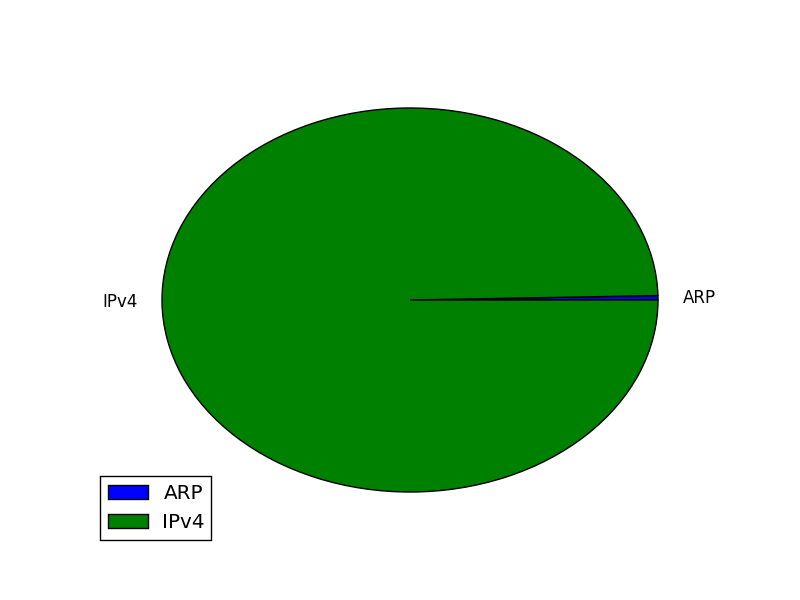
\includegraphics[width=0.5\textwidth]{plot/laboDcS-pie.png}
        \caption{Labos Dc - Probabilidades}
        \label{torta:labosDcS}
    \end{center}
\end{figure}

La entropía de la fuente $S$ fue de 0.034922 lo que hace que los símbolos emitidos por la fuente $S$ sean muy previsibles como podemos notarlo en la figura~\ref{histo:laboDcS} donde observamos que la información aportada por el protocolo IPv4 se encuentra por debajo de la entropía de $S$. El protocolo ARP aporta información muy por arriba de la entropía como se observa en la figura~\ref{histo:laboDcS} pero según lo observado en la figura~\ref{torta:labosDcS} tiene una probabilidad demasiado baja lo que hace que no incida en la entropía.

\begin{figure}[H]
    \begin{center}
        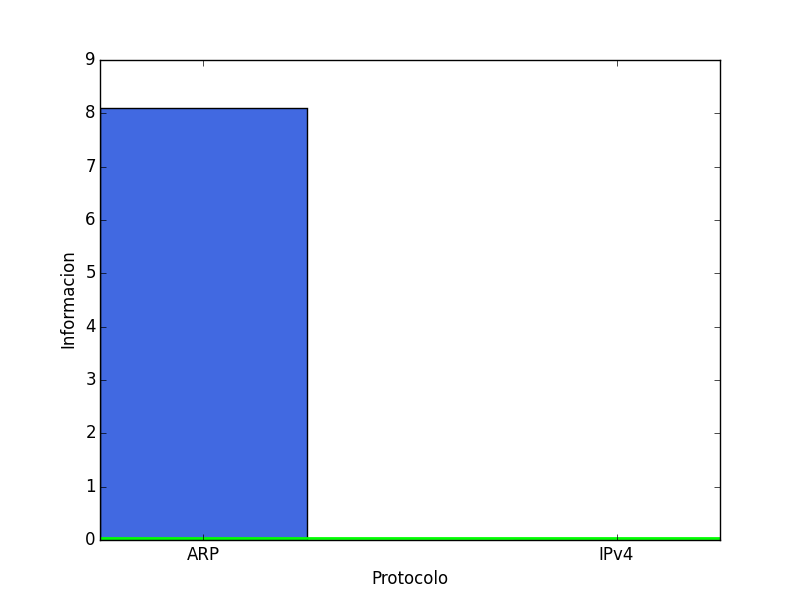
\includegraphics[width=0.5\textwidth]{plot/laboDcS-bar.png}
        \caption{Labos Dc - Información}
        \label{histo:laboDcS}
    \end{center}
\end{figure}

\subsubsection{Fuente $S_1$}

Para la fuente $S_1$ expondremos las ip de destino. Dala la cantidad de ips capturadas para facilitar la lectura de los gráficos y tablas expondremos 2 bloques (A yB) en representación de ips de destino que tuvieron igual aporte de información en la captura. Para el caso del bloque A se compone de 19 ip con igual aporte de información y el bloque B de 7 ips. Los resultados fueron :

\begin{table}[H]
    \begin{center}
        \begin{tabular}{|c|c|c|}
            \hline
            \textbf{Protocolo} & \textbf{Información} & \textbf{Probabilidad} \\ \hline
            \texttt{A(19 ips)}    &8.40        & 5.60\%     \\ \hline
            \texttt{B(7 ips)}     &7.40        & 4.13\%     \\ \hline
            \texttt{10.2.203.144} &6.82        & 0.88\%     \\ \hline
            \texttt{10.2.202.5}   &6.82        & 0.88\%     \\ \hline
            \texttt{10.2.202.228} &6.82        & 0.88\%     \\ \hline
            \texttt{10.2.203.122} &6.40        & 1.17\%     \\ \hline
            \texttt{10.2.203.117} &6.40        & 1.17\%     \\ \hline
            \texttt{10.2.203.254} &4.82        & 3.53\%     \\ \hline
            \texttt{10.2.201.214} &4.23        & 5.30\%     \\ \hline
            \texttt{10.2.202.132} &4.08        & 5.89\%     \\ \hline
            \texttt{10.2.200.217} &4.01        & 6.19\%     \\ \hline
            \texttt{10.2.202.108} &2.33        & 19.76\%     \\ \hline
            \texttt{10.2.202.100} &2.33        & 19.76\%     \\ \hline
            \texttt{10.2.202.47}  &2.01        & 24.77\%     \\ \hline   
        \end{tabular}
        \caption{Labos Dc - Nodos}
        \label{table:laboDcS1}
    \end{center}
\end{table}

Como puede observarse en la figura~\ref{torta:laboDcS1} las ip que aparecen con mayor frecuencia como destino en los paquetes ARP son la ``10.2.202.47'' en un 24.77\%, la ``10.2.202.100'' en un 19.76\% y la ``10.2.202.108'' en un 19.76\% por lo que estas serán los nodos distinguidos de la fuente y las que menos información aporten.

\begin{figure}[H]
    \begin{center}
        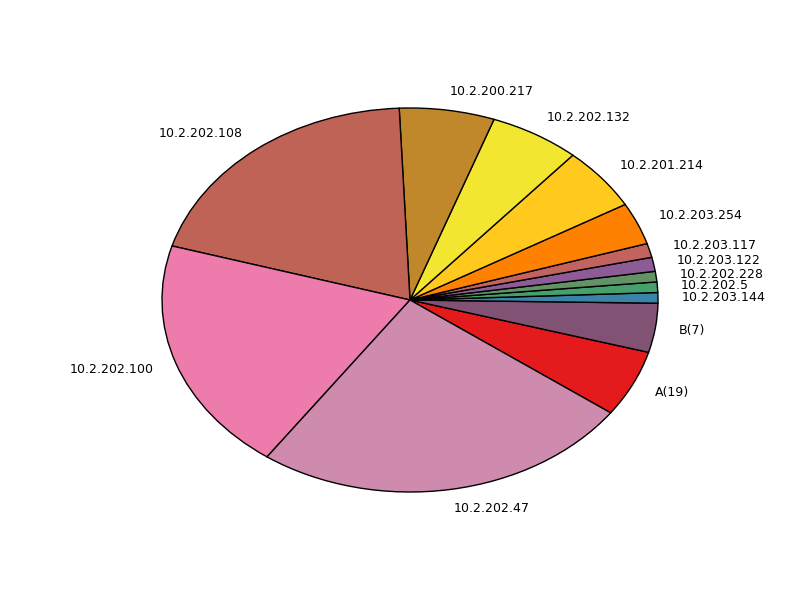
\includegraphics[width=0.5\textwidth]{plot/laboDcS1-pie.png}
        \caption{Labos Dc - Probabilidades}
        \label{torta:laboDcS1}
    \end{center}
\end{figure} 

La entropía de la fuente $S_1$ fue de 3.417440. En la figura~\ref{histo:laboDcS1} se observa la información aportada por los distintos nodos y como los 3 nodos distinguidos quedan por debajo de la entropía de la fuente. 

\begin{figure}[H]
    \begin{center}
        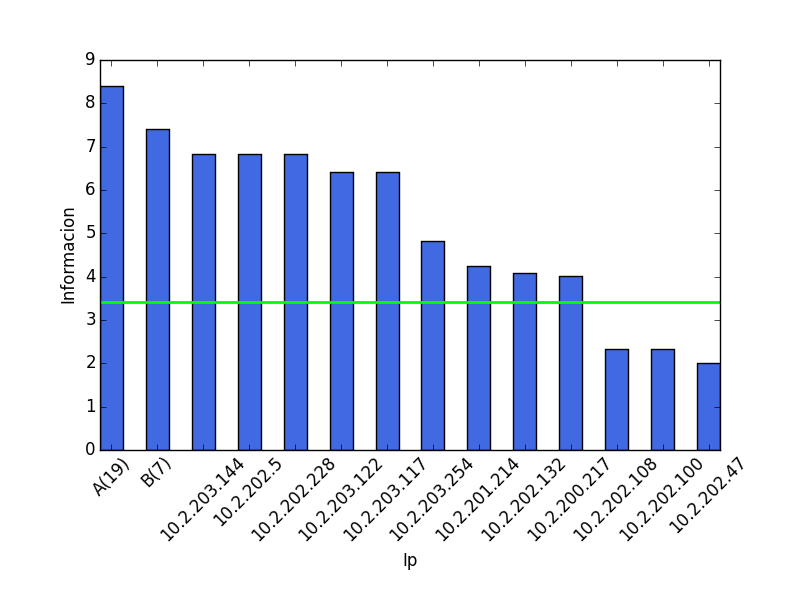
\includegraphics[width=0.5\textwidth]{plot/laboDcS1-bar.png}
        \caption{Labos Dc - Información}
        \label{histo:laboDcS1}
    \end{center}
\end{figure}

En el análisis de la fuente $S_1$ vemos que ninguno de los 3 nodos distinguidos pertenecen al router de la red, la ip ``10.2.203.254'' ni tampoco a la ip de la maquina que realizo la captura ``10.2.202.132''. No tenemos información de la red para precisar a que pertencen las ip de los nodos distinguidos.

%%%%%%%%%%%%%%%%%%%%%%%%%%%%%%%%%%%%%%%%%%%%%%%%%%%%%%%%
%%%%%%%%%%%%%%%%%%%%%%%%%%%%%%%%%%%%%%%%%%%%%%%%%%%%%%%%
%%%%%%%%%%%%%%%%%%%%%%%%%%%%%%%%%%%%%%%%%%%%%%%%%%%%%%%%
%%%%%%%%%%%%%%%%%%%%%%%%%%%%%%%%%%%%%%%%%%%%%%%%%%%%%%%%


\subsection{Zona pública (parque)}
\subsubsection{Fuente S}

Los resultados obtenidos para la fuente $S$ fueron:

\begin{table}[H]
    \begin{center}
        \begin{tabular}{|c|c|c|}
            \hline
            \textbf{Protocolo} & \textbf{Información} & \textbf{Probabilidad} \\ \hline
            \texttt{IPv6      }& 1.763        & 29.45\%    \\ \hline
            \texttt{ARP       }& 1.646        & 31.95\%     \\ \hline
            \texttt{IPv6      }& 1.373        & 38.59\%    \\ \hline
        \end{tabular}
        \caption{Zona Pública (parque) - Protocolos}
        \label{table:parqueS}
    \end{center}
\end{table} 

Podemos notar en la figura~\ref{torta:parqueS} que el protocolo más utilizado es IPv4 (38.5919\%) seguido por ARP (31.9503\%) e IPv6 (29.4578\%). En comparación con las redes analizadas en secciones anteriores, los paquetes ARP son muy frecuentes. Otra peculiaridad es que el protocolo IPv4 y el IPv6 son usados en casi la misma frecuencia, lo que no sucedió en las redes anteriores.

\begin{figure}[H]
    \begin{center}
        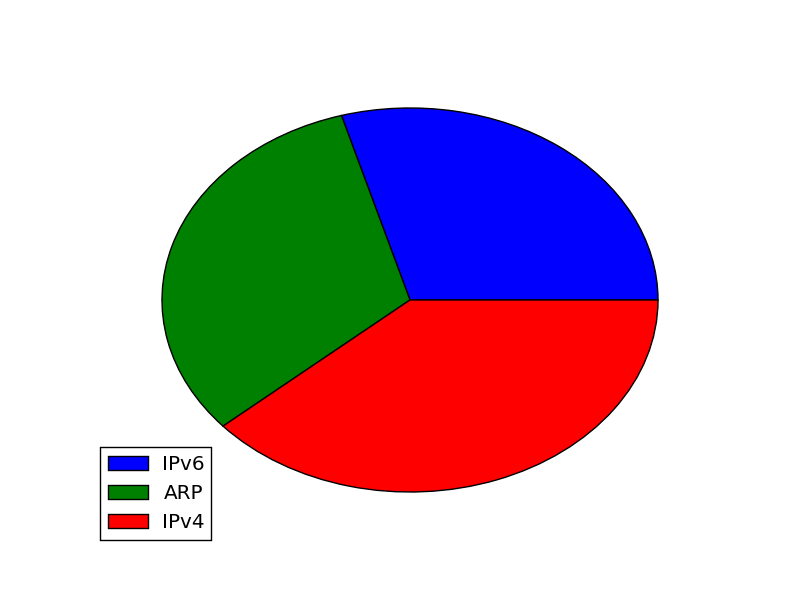
\includegraphics[width=0.5\textwidth]{plot/parqueS-pie.png}
        \caption{Zona Pública (parque) - Probabilidades}
        \label{torta:parqueS}
    \end{center}
\end{figure}

En cuanto a la entropía de la fuente $S$, fue de $1.575466$, lo que nos dice que los símbolos emitidos por la fuente no son previsibles, ya que ningún protocolo otorga mucha más información que los demás (ver figura~\ref{histo:parqueS}). No podemos decir que para esta fuente haya un símbolo distinguido en esta fuente.

\begin{figure}[H]
    \begin{center}
        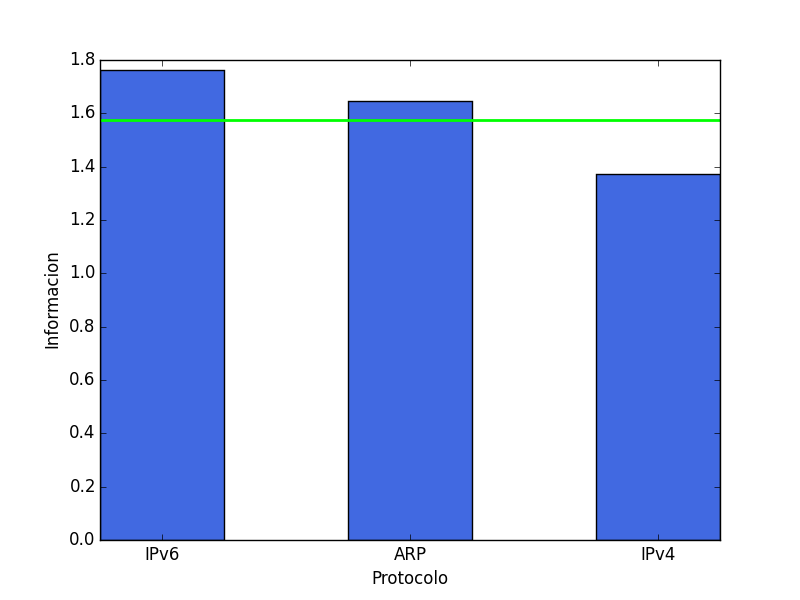
\includegraphics[width=0.5\textwidth]{plot/parqueS-bar.png}
        \caption{Zona Pública (parque) - Informacion}
        \label{histo:parqueS}
    \end{center}
\end{figure}

\subsubsection{Fuente $S_1$}

Para la fuente $S_1$ expondremos las ip de destino. Dada la cantidad de ips capturadas, para facilitar la lectura de los gráficos y tablas, expondremos las direcciones ip que tuvieron igual aporte de información en la captura en bloques.

\begin{table}[H]
    \begin{center}
        \begin{tabular}{|c|c|c|}
            \hline
            \textbf{Protocolo} & \textbf{Información} & \textbf{Probabilidad} \\ \hline
            \texttt{B1(171 ips)}    &14.105417        & 0.97\%     \\ \hline
            \texttt{B2(227 ips)}    &13.105417        & 2.56\%     \\ \hline
            \texttt{B3(348 ips)}    &12.422595        & 6.38\%     \\ \hline
            \texttt{B4(253 ips)}    &11.601712        & 8.25\%     \\ \hline
            \texttt{B5(40 ips)}     &10.649047        & 2.53\%     \\ \hline
            \texttt{B6(16 ips)}     &9.504669         & 2.25\%     \\ \hline       
            \texttt{B7(4 ips)}      &8.569523         & 1.06\%     \\ \hline
            \texttt{B8(5 ips)}      &7.543969         & 2.69\%     \\ \hline
            \texttt{B9(4 ips)}      &6.495808         & 4.49\%     \\ \hline
            \texttt{169.254.255.255} &5.380904        & 2.39\%     \\ \hline 
            \texttt{10.249.147.254} &4.970991         & 3.18\%     \\ \hline 
            \texttt{10.248.79.254} &4.908201          & 3.33\%     \\ \hline 
            \texttt{10.248.0.100} &4.340546           & 4.93\%     \\ \hline 
            \texttt{10.248.0.68} &4.277281            & 5.15\%     \\ \hline 
            \texttt{10.249.111.254} &4.129570         & 5.71\%     \\ \hline 
            \texttt{10.248.255.254} &3.972275         & 6.37\%     \\ \hline 
            \texttt{169.254.188.151} &3.521395        & 8.70\%     \\ \hline 
            \texttt{10.249.107.249} &3.278075         &10.30\%     \\ \hline 
            \texttt{10.250.127.254} &2.422862         &18.64\%     \\ \hline
        \end{tabular}
        \caption{Zona publica (parque) - Nodos}
        \label{table:parqueS1}
    \end{center}
\end{table}

La entropía de la fuente fue de $5.757719$, lo que indica que la fuente tiene un alto nivel de imprevisivilidad. Podemos ver que los bloques de direcciones de B1 a B14 son nodos diferenciados debido a la alta cantidad de información aportada, es decir, su baja probabilidad de aparecer como símbolo en la fuente; de la misma manera, las direcciones ip \texttt{10.249.107.249} y \texttt{10.250.127.254} también se diferencian pero por la razón contraria, aportan muy poca información, por tener una frecuencia relativa de aparición alta durante las capturas en relación a los otros símbolos.

\begin{figure}[H]
    \begin{center}
        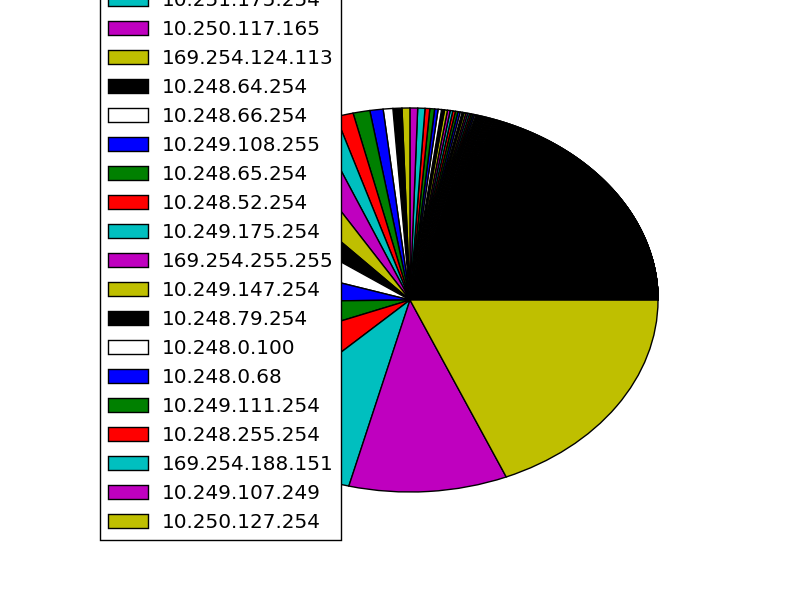
\includegraphics[width=0.5\textwidth]{plot/parqueS1-pie.png}
        \caption{Parque S1 - Probabilidades}
        \label{torta:parqueS1}
    \end{center}
\end{figure} 

\begin{figure}[H]
    \begin{center}
        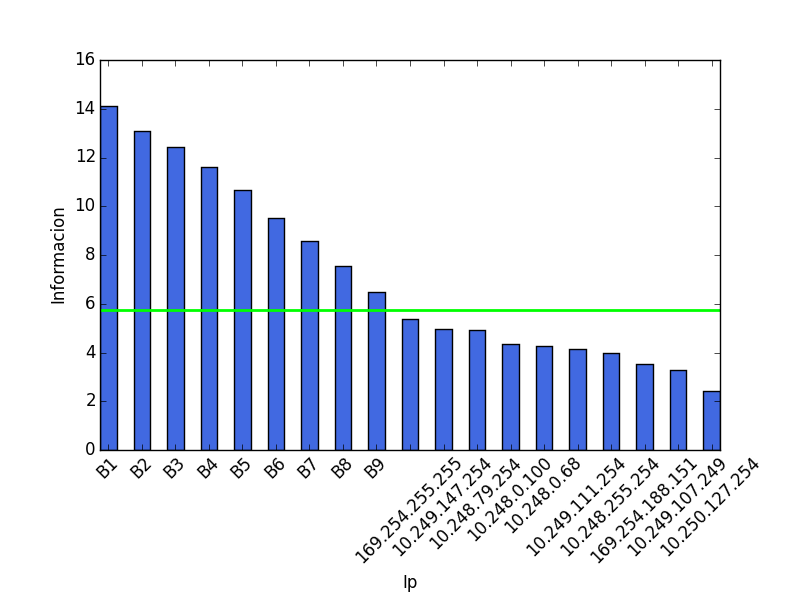
\includegraphics[width=0.5\textwidth]{plot/parqueS1-bar.png}
        \caption{Parque - Información}
        \label{histo:parqueS1}
    \end{center}
\end{figure}

Como particularidad en esta red observamos la presencia de nodos con ips fuera del rango usado por la red como ser la ip 169.255.188.151. Estas ip pertenecen a nodos que no tienen una ip asignada en la red y estan usando como ip la asignada por ``ipv4ll'' mediante ``zeroconf''. Esta tecnologia asigna una ip automáticamente cuando el nodo no puede obtener una ip a traves de DHCPCD o no tiene configurada una ip fija. Las ips asignadas de esta manera pertenecen al bloque de ips 169.254.0.0/16.

\subsection{Universidad de La Matanza}
\subsubsection{Fuente S}

Los resultados obtenidos para la fuente $S$ fueron:

\begin{table}[H]
    \begin{center}
        \begin{tabular}{|c|c|c|}
            \hline
            \textbf{Protocolo} & \textbf{Información} & \textbf{Probabilidad} \\ \hline
            \texttt{IPv6      }& 6.753        & 0.009\%     \\ \hline
            \texttt{ARP       }& 1.269        & 0.415\%     \\ \hline
	    \texttt{IPv4      }& 0.796        & 0.576\%     \\ \hline
        \end{tabular}
        \caption{Universidad de La Matanza - Protocolos}
        \label{table:universidadLMS}
    \end{center}
\end{table} 

Se observa en la figura~\ref{torta:universidadLMS} que los protocolos más utilizados son IPv4 en un 57.60\% y ARP con un 41.50\%, el uso del protocolo IPv6 es de apenas 0.9%. La cantidad de mensajes ARP es bastante elevado para esta red, creemos que esto podría indicar una gran variabilidad de los componentes conectados (dispositivos que se conectan por poco tiempo). El uso despreciable del protocolo IPv6 creemos que podría justificarse por un tema de configuración propia de la red.

\begin{figure}[H]
    \begin{center}
        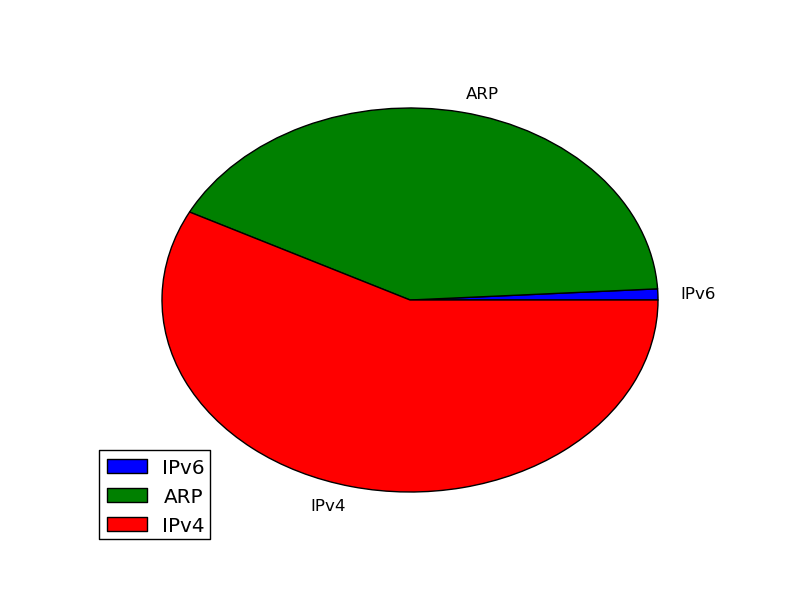
\includegraphics[width=0.5\textwidth]{plot/facultadS-pie.png}
        \caption{Universidad de La Matanza - Probabilidades}
        \label{torta:universidadLMS}
    \end{center}
\end{figure}

La entropía de la fuente $S$ fue de 1.047737 lo que hace que los símbolos emitidos por la fuente $S$ sean muy imprevisibles como podemos notarlo en la figura~\ref{histo:universidadLMS} donde observamos que la información aportada por el protocolo IPv4 se parece a la del protocolo ARP ambos muy cerca de la entropía de $S$. El protocolo IPv6 aporta información muy por arriba de la entropía según la figura~\ref{histo:universidadLMS}, pero según lo observado en la figura~\ref{torta:universidadLMS} tiene una probabilidad demasiado baja lo que hace que no incida en la entropía.

\begin{figure}[H]
    \begin{center}
        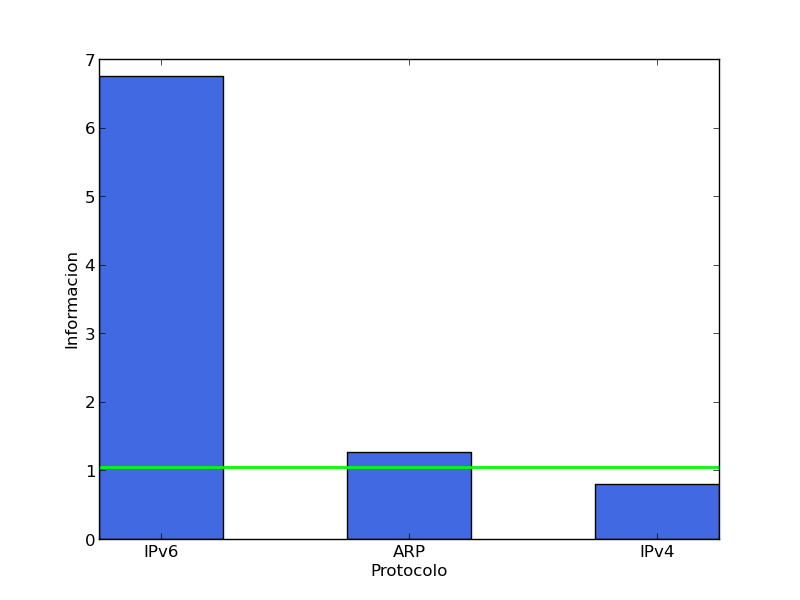
\includegraphics[width=0.5\textwidth]{plot/facultadS-bar.png}
        \caption{Universidad de La Matanza - Información}
        \label{histo:universidadLMS}
    \end{center}
\end{figure}

\subsubsection{Fuente $S_1$}

Para la fuente $S_1$ expondremos las ip de destino. Dada la cantidad de ips capturadas para facilitar la lectura de los gráficos y tablas expondremos varios bloques de (A hasta I) en representación de ips de destino que tuvieron un aporte de información parecido en la captura. Como había demasiadas ips, para las que estaban muy por encima de la entropía se utilizo un promedio para darle un valor para el gráfico. Los resultados fueron :

\begin{table}[H]
    \begin{center}
        \begin{tabular}{|c|c|c|}
            \hline
            \textbf{Protocolo} & \textbf{Información} & \textbf{Probabilidad} \\ \hline
            \texttt{A(131 ips)}   &13.450309       & 1.16\%     \\ \hline
            \texttt{B(74 ips)}    &12.450309       & 1.32\%     \\ \hline
            \texttt{C(155 ips)}   &11.540077       & 5.31\%     \\ \hline
	        \texttt{D(77 ips)}    &10.565611       & 5.16\%     \\ \hline
	        \texttt{E(103 ips)}   &9.564986        & 13.86\%    \\ \hline
            \texttt{F(38 ips)}    &8.755480        & 8.83\%     \\ \hline
    	    \texttt{G(38 ips)}    &8.271055        & 12.36\%    \\ \hline
	        \texttt{H(28 ips)}    &7.732110        & 13.23\%    \\ \hline
	        \texttt{I(20 ips)}    &7.272395        & 12.99\%    \\ \hline
            \texttt{10.5.83.154}  &6.990878        & 0.78\%    \\ \hline
            \texttt{10.5.73.140}  &6.974576        & 0.79\%    \\ \hline
            \texttt{10.5.78.34}   &6.942515        & 0.81\%    \\ \hline
            \texttt{169.254.255.255} &6.895720     & 0.83\%    \\ \hline
            \texttt{10.5.77.136}  &6.865347        & 0.85\%    \\ \hline
            \texttt{10.5.82.0}    &6.668949        & 0.98\%    \\ \hline
            \texttt{10.5.84.63}   &6.579944        & 1.04\%    \\ \hline
            \texttt{10.5.70.239}  &6.543419        & 1.07\%    \\ \hline
            \texttt{10.5.70.216}  &6.119392        & 1.43\%    \\ \hline
            \texttt{10.5.80.111}  &6.024044        & 1.53\%    \\ \hline
            \texttt{10.5.200.13}  &5.911150        & 1.66\%    \\ \hline
            \texttt{10.5.77.177}  &5.784973        & 1.81\%    \\ \hline
            \texttt{10.5.0.1}     &5.531446        & 2.16\%    \\ \hline
            \texttt{10.5.80.17}   &5.455956        & 2.27\%    \\ \hline
            \texttt{10.5.103.253} &3.707158        & 7.65\%    \\ \hline    
        \end{tabular}
        \caption{Universidad de La Matanza - Nodos}
        \label{table:universidadLMS1}
    \end{center}
\end{table}

Como puede observarse en la figura~\ref{torta:universidadLMS1} las ip que aparecen con mayor frecuencia como destino en los paquetes ARP son la ``10.5.103.253'' en un 7.65\%, la ``10.5.80.17'' en un 2.27\%, ``10.5.0.1'' en un 2.16\%, la ``10.5.77.177'' en un 1.81\%, la ``10.5.200.13'' en un 1.66\%, la ``10.5.70.216'' en un 1.43\% y varias mas, por lo que estas serán los nodos distinguidos de la fuente y las que menos información aporten.

\begin{figure}[H]
    \begin{center}
        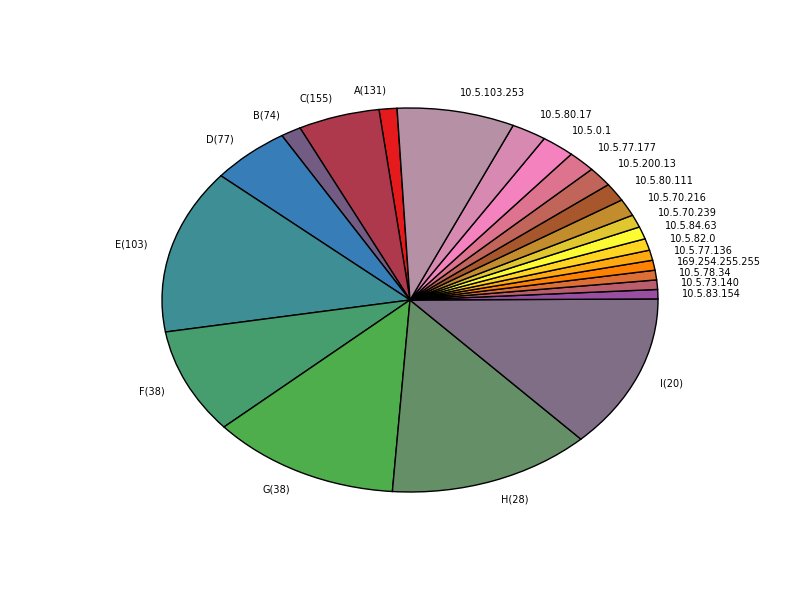
\includegraphics[width=0.5\textwidth]{plot/facultadS1-pie.png}
        \caption{Universidad de La Matanza - Probabilidades}
        \label{torta:universidadLMS1}
    \end{center}
\end{figure} 

La entropía de la fuente $S_1$ fue de 7.951183. En la figura~\ref{histo:universidadLMS1} y la figura ~\ref{torta:universidadLMS1} se observa la información aportada por los distintos nodos y como los 4 nodos distinguidos quedan por debajo de la entropía de la fuente. En este caso había muchas ips por debajo de la entropía (casí 30 ips), así que tomamos como punto de corte los que tengan una probabilidad mayor a 1%.

\begin{figure}[H]
    \begin{center}
        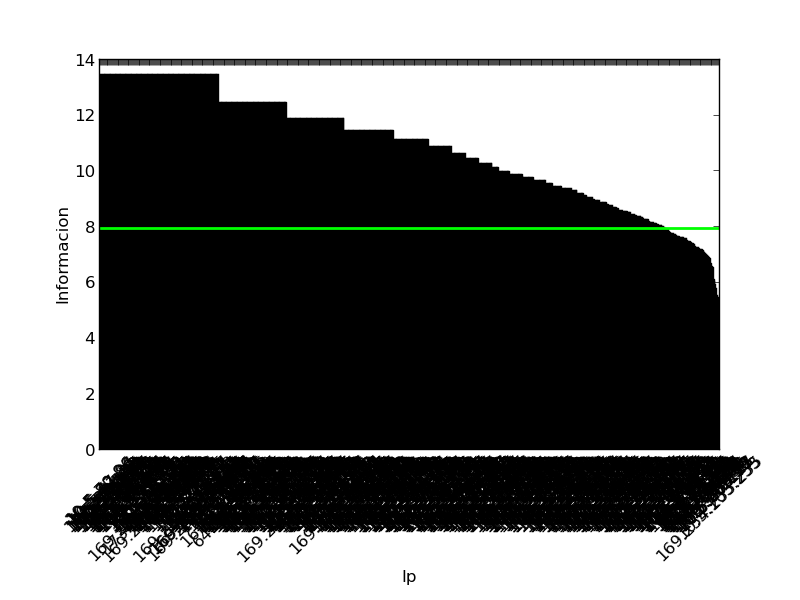
\includegraphics[width=0.5\textwidth]{plot/facultadS1-bar.png}
        \caption{Universidad de La Matanza - Información}
        \label{histo:universidadLMS1}
    \end{center}
\end{figure}

En el análisis de la fuente $S_1$ vemos que la ip ``10.5.0.1'' podría corresponderse algún router y de los otros 3 nodos no disponemos de suficiente información sobre la red para saber cual es el rol que cumplen.

\section{Conclusión}
En este trabajo se analizaron 4 redes distintas desde el punto de vista de la teoría de la información. Este enfoque nos permitió distinguir y cuantificar la importancia de distintos entes dentro de las redes , ya sean protocolos y su uso relativo en las redes LAN analizadas o nodos que las conforman. (FALTA UNA RED PARA LAS CONCLUSIONES)


\section{Referencias}

\end{document}
